
\documentclass[11pt,a4paper,UTF8]{ctexart}

\usepackage[T1]{fontenc}
\usepackage[utf8]{inputenc}
\usepackage{authblk}

\usepackage{ctex} %导入中文包
\usepackage{tocvsec2}

\usepackage{tabularx}
\usepackage{booktabs} 
\usepackage{multirow}
\usepackage{bbding}
\usepackage{float}
\usepackage{xspace}

\usepackage{graphicx}
\usepackage{subfigure}

\usepackage{subfiles} %使用多文件方式进行

\usepackage{geometry} %设置页边距的包
\geometry{left=2.5cm,right=2cm,top=2.54cm,bottom=2.54cm} %设置书籍的页边距

\usepackage{hyperref}  %制作pdf的目录
\hypersetup{hidelinks, %去红框
	colorlinks=true,
	allcolors=black,
	pdfstartview=Fit,
	breaklinks=true
}

% 调整itemlist中的行间距
\usepackage{enumitem}
\setenumerate[1]{itemsep=0pt,partopsep=0pt,parsep=\parskip,topsep=5pt}
\setitemize[1]{itemsep=0pt,partopsep=0pt,parsep=\parskip,topsep=5pt}
\setdescription{itemsep=0pt,partopsep=0pt,parsep=\parskip,topsep=5pt}

% 超链接样式设置
\usepackage{hyperref}
\hypersetup{
	colorlinks=true,
	linkcolor=blue,
	filecolor=blue,
	urlcolor=blue,
	citecolor=cyan,
}

\usepackage{indentfirst}

\usepackage{listings}
\usepackage[usenames,dvipsnames,svgnames, x11names]{xcolor}

\usepackage{tcolorbox}

%展示代码
\definecolor{mygreen}{rgb}{0,0.6,0}
\definecolor{mygray}{rgb}{0.5,0.5,0.5}
\definecolor{mymauve}{rgb}{0.58,0,0.82}
\lstset{
	backgroundcolor=\color{blue!3!white}, 
	basicstyle = \footnotesize,       
	breakatwhitespace = false,        
	breaklines = true,                 
	captionpos = b,                    
	commentstyle = \color{mygreen}\bfseries,
	extendedchars = false,             
	frame =shadowbox, 
	framerule=0.5pt,
	keepspaces=true,
	keywordstyle=\color{blue}\bfseries, % keyword style
	language = C++,                     % the language of code
	otherkeywords={string}, 
	numbers=left, 
	numbersep=5pt,
	numberstyle=\tiny\color{mygray},
	rulecolor=\color{black},         
	showspaces=false,  
	showstringspaces=false, 
	showtabs=false,    
	stepnumber=1,         
	stringstyle=\color{mymauve},        % string literal style
	tabsize=2,          
	title=\lstname                      
}

\begin{document}
	%\maketitle
	
	\begin{center}
		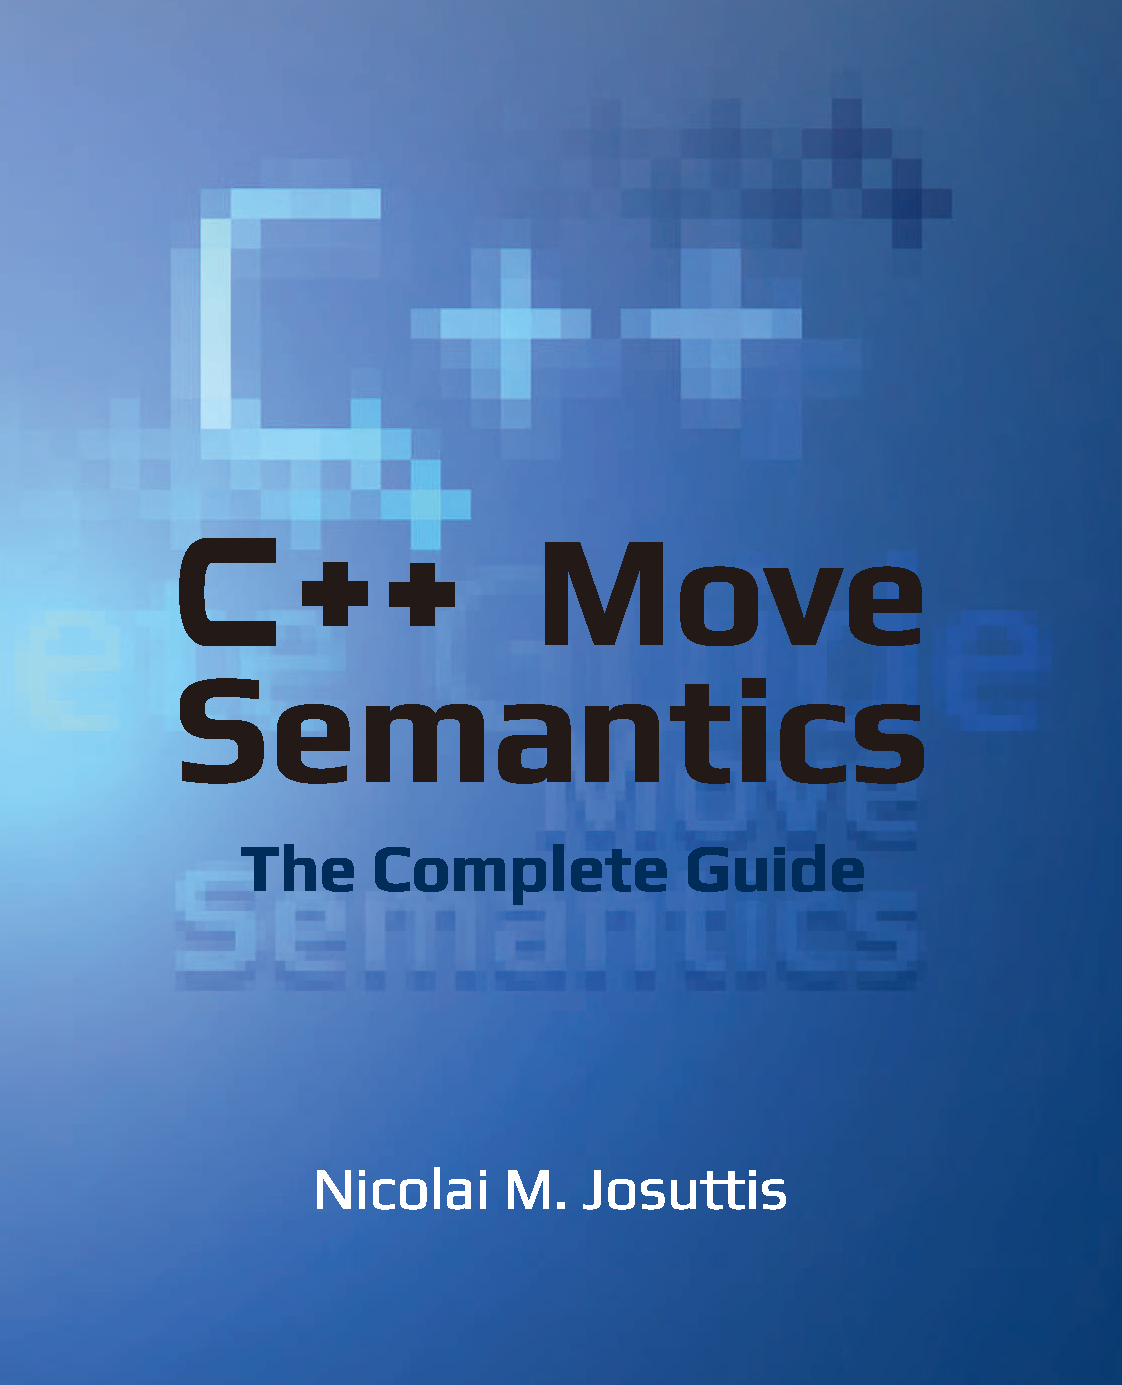
\includegraphics[width=1.\textwidth]{cover}
		\newpage
		\huge
		\textbf{C++ Move Semantics} 
		\\[9pt]
		\normalsize
		The Complete Guide
		\\[10pt]
		\normalsize 
		作者: Nicolai M. Josuttis
		\\[8pt]
		\normalsize
		译者;陈晓伟
	\end{center}
	
	\hspace*{\fill} \\ %插入空行
	\noindent\textbf{本书概述}\ \par

	完整的介绍C++ Move语义。\par
	
	C++11添加的Move语义已经成为现代C++的标志,也使语言变得复杂,即使经验丰富的开发者仍在需要仔细处理Move语义的细节。因为这个原因,一些编程书籍甚至不推荐对非常简单的类使用Move语义。所以,详细的解释C++ Move语义就变得刻不容缓。\par
	
	本书会从基本原理开始来介绍Move语义,并会解释Move语义的所有细节,使每个开发者都可以正确地使用Move语义。\par
	
	本书项目始于2019年,对于完全支持C++和数据并行的需要大量的扩展,超出当时的SYCL 1.2.1标准。DPC++编译器需要支持这些扩展,包括对统一共享内存(USM)的支持、通过SYCL完成三级层次结构的子工作组、匿名Lambda和许多编程简化。\par
	
	你将学习到:\par
	
	\begin{itemize}
		\item Move语义的起因和术语
		\item 如何隐式地获益于Move语义
		\item 如何明确地获益于Move语义
		\item 会遇到的所有问题,以及如何处理它们
		\item 所有的结果都取决于你的编程风格
	\end{itemize}
	
	重点在于所描述的特性,需要在实践中进行应用。示例和背景信息,有助于理解和改进简单类,甚至泛型库和框架的代码。\par
	
	“我以为我理解了Move的语义,但我真的不懂!”我从你的书中学到了很多东西。”	-- Jonathan Boccara\par
	
	“这是我需要很久的书。” -- Rob Bernstein\par
	
	“有时候我觉得我对纠缠和量子隐形传态的理解,要比我对一些奇怪的C++ Move语义的理解要好。套用Feynman的话:如果你认为你理解了C++的Move语义,那你就不理解C++的Move语义。赶快阅读这本书吧。”	-- Victor Ciura\par
	
	
	\hspace*{\fill} \\ %插入空行
	\noindent\textbf{作者简介}\ \par
	Nicolai Josuttis (http://www.josuttis.com)在编程界很有名,因为他的发言和著作都很有权威,还是世界范围内畅销书的(共同)作者:\par
	
	\begin{itemize}
		\item 《The C++ Standard Library》
		\item 《C++ Templates》
		\item 《C++ Move Semantics》
		\item 《C++17》
		\item 《SOA in Practice》
	\end{itemize}
	
	同时也是一位富有创新精神的演讲者,曾在各种会议和活动中发言。还是独立的讲师,并且在C++标准化方面有20多年的经验。\par
	
	\hspace*{\fill} \\ %插入空行
	\noindent\textbf{本书相关}\ \par
	\begin{itemize}
		\item github翻译地址:\href{https://github.com/xiaoweiChen/CPP-Move-Semantics}{https://github.com/xiaoweiChen/CPP-Move-Semantics}
	\end{itemize}
	\newpage
	
	\tableofcontents
	\newpage
	
	%前言和关于本书
	\pagestyle{empty}
	\subfile{content/Preface.tex}
	\subfile{content/About_This_Book.tex}

	\setsecnumdepth{section}
	\section{Part I: 移动语义的基本特征}
	\subfile{content/1/Part-1.tex}
	\subsection{1 移动语义的力量}
	\subfile{content/1/chapter1/0.tex}
		\subsubsection{1.1 设计移动语义的动机}
		\subfile{content/1/chapter1/1.tex}
		\subsubsection{1.2 实现移动语义}
		\subfile{content/1/chapter1/2.tex}
		\subsubsection{1.3 复制是一种应急方式}
		\subfile{content/1/chapter1/3.tex}
		\subsubsection{1.4 const对象的移动语义}
		\subfile{content/1/chapter1/4.tex}
		\subsubsection{1.5 总结}
		\subfile{content/1/chapter1/5.tex}
	\subsection{2 移动语义的核心}
	\subfile{content/1/chapter2/0.tex}
		\subsubsection{2.1 右值引用}
		\subfile{content/1/chapter2/1.tex}
		\subsubsection{2.2 std::move()}
		\subfile{content/1/chapter2/2.tex}
		\subsubsection{2.3 移动的对象}
		\subfile{content/1/chapter2/3.tex}
		\subsubsection{2.4 通过引用进行重载}
		\subfile{content/1/chapter2/4.tex}
		\subsubsection{2.5 按值传递}
		\subfile{content/1/chapter2/5.tex}
		\subsubsection{2.6 总结}
		\subfile{content/1/chapter2/6.tex}
	\subsection{3 类中的移动语义}
	\subfile{content/1/chapter3/0.tex}
		\subsubsection{3.1 普通类中移动语义}
		\subfile{content/1/chapter3/1.tex}
		\subsubsection{3.2 实现复制/移动函数}
		\subfile{content/1/chapter3/2.tex}
		\subsubsection{3.3 特殊成员函数的规则}
		\subfile{content/1/chapter3/3.tex}
		\subsubsection{3.4 三五法则}
		\subfile{content/1/chapter3/4.tex}
		\subsubsection{3.5 总结}
		\subfile{content/1/chapter3/5.tex}
	\subsection{4 如何从移动语义中获益}
	\subfile{content/1/chapter4/0.tex}
		\subsubsection{4.1 避免命名对象}
		\subfile{content/1/chapter4/1.tex}
		\subsubsection{4.2 避免不必要的std::move()}
		\subfile{content/1/chapter4/2.tex}
		\subsubsection{4.3 用移动语义初始化成员}
		\subfile{content/1/chapter4/3.tex}
		\subsubsection{4.4 类中使用移动语义}
		\subfile{content/1/chapter4/4.tex}
		\subsubsection{4.5 总结}
		\subfile{content/1/chapter4/5.tex}
	\subsection{5 引用的重载}
	\subfile{content/1/chapter5/0.tex}
		\subsubsection{5.1 getter的返回类型}
		\subfile{content/1/chapter5/1.tex}
		\subsubsection{5.2 重载}
		\subfile{content/1/chapter5/2.tex}
		\subsubsection{5.3 何时使用引用}
		\subfile{content/1/chapter5/3.tex}
		\subsubsection{5.4 总结}
		\subfile{content/1/chapter5/4.tex}
	\subsection{6 已移动状态}
	\subfile{content/1/chapter6/0.tex}
		\subsubsection{6.1 已移动对象的要求和状态}
		\subfile{content/1/chapter6/1.tex}
		\subsubsection{6.2 可销毁和可转移}
		\subfile{content/1/chapter6/2.tex}
		\subsubsection{6.3 处理已破坏的不变量}
		\subfile{content/1/chapter6/3.tex}
		\subsubsection{6.4 总结}
		\subfile{content/1/chapter6/4.tex}
	\subsection{7 移动语义和noexcept}
	\subfile{content/1/chapter7/0.tex}
		\subsubsection{7.1 移动构造函数有和没有noexcept的区别}
		\subfile{content/1/chapter7/1.tex}
		\subsubsection{7.2 noexcept声明的细节}
		\subfile{content/1/chapter7/2.tex}
		\subsubsection{7.3 noexcept在类中的声明}
		\subfile{content/1/chapter7/3.tex}
		\subsubsection{7.4 何时何地使用noexcept}
		\subfile{content/1/chapter7/4.tex}
		\subsubsection{7.5 总结}
		\subfile{content/1/chapter7/5.tex}
	\subsection{8 值的种类}
	\subfile{content/1/chapter8/0.tex}
		\subsubsection{8.1 值的种类}
		\subfile{content/1/chapter8/1.tex}
		\subsubsection{8.2 值类别的特殊规则}
		\subfile{content/1/chapter8/2.tex}
		\subsubsection{8.3 绑定引用时值类别的影响}
		\subfile{content/1/chapter8/3.tex}
		\subsubsection{8.4 当左值变成右值}
		\subfile{content/1/chapter8/4.tex}
		\subsubsection{8.5 当右值变成左值}
		\subfile{content/1/chapter8/5.tex}
		\subsubsection{8.6 使用decltype检查值类别}
		\subfile{content/1/chapter8/6.tex}
		\subsubsection{8.7 总结}
		\subfile{content/1/chapter8/7.tex}
		
	\section{Part II: 泛型代码中的移动语义}
	\subfile{content/2/Part-2.tex}
	\subsection{9 完美转发}
	\subfile{content/2/chapter9/0.tex}
		\subsubsection{9.1 完美转发的动机}
		\subfile{content/2/chapter9/1.tex}
		\subsubsection{9.2 实现完美转发}
		\subfile{content/2/chapter9/2.tex}
		\subsubsection{9.3 右值引用与通用引用}
		\subfile{content/2/chapter9/3.tex}
		\subsubsection{9.4 使用通用引用的重载}		
		\subfile{content/2/chapter9/4.tex}
		\subsubsection{9.5 Lambda中的完美转发}
		\subfile{content/2/chapter9/5.tex}
		\subsubsection{9.6 总结}
		\subfile{content/2/chapter9/6.tex}
	\subsection{10 完美转发的细节}
	\subfile{content/2/chapter10/0.tex}
		\subsubsection{10.1 通用引用作为非转发引用}
		\subfile{content/2/chapter10/1.tex}
		\subsubsection{10.2 通用或普通rvalue引用?}
		\subfile{content/2/chapter10/2.tex}
		\subsubsection{10.3 C++标准如何指定完美转发}
		\subfile{content/2/chapter10/3.tex}
		\subsubsection{10.4 完美转发(不美丽的)细节}
		\subfile{content/2/chapter10/4.tex}
		\subsubsection{10.5 总结}
		\subfile{content/2/chapter10/5.tex}
	\subsection{11 用auto\&\&完美传递}
	\subfile{content/2/chapter11/0.tex}
		\subsubsection{11.1 默认的完美的传递}
		\subfile{content/2/chapter11/1.tex}
		\subsubsection{11.2 使用auto\&\&的通用引用}
		\subfile{content/2/chapter11/2.tex}
		\subsubsection{11.3 auto\&\&的非转发引用}
		\subfile{content/2/chapter11/3.tex}
		\subsubsection{11.4 完美的Lambda转发}
		\subfile{content/2/chapter11/4.tex}
		\subsubsection{11.5 C++20中函数声明使用auto\&\&}
		\subfile{content/2/chapter11/5.tex}
		\subsubsection{11.6 总结}
		\subfile{content/2/chapter11/6.tex}
	\subsection{12 完美返回decltype(auto)}
	\subfile{content/2/chapter12/0.tex}
		\subsubsection{12.1 完美返回}
		\subfile{content/2/chapter12/1.tex}
		\subsubsection{12.2 decltype(auto)}
		\subfile{content/2/chapter12/2.tex}
		\subsubsection{12.3 总结}
		\subfile{content/2/chapter12/3.tex}
		
	\section{Part III: Move Semantics in the C++ Standard Library}
	\subsection{13 Move-Only Types}
	%\subfile{content/chapter-13/13-0.tex}
		\subsubsection{13.1 Declaring and Using Move-Only Types}
		%\subfile{content/chapter-13/13-1.tex}
		\subsubsection{13.2 总结}
		%\subfile{content/chapter-13/13-10.tex}
	\subsection{14 Moving Algorithms and Iterators}
	%\subfile{content/chapter-14/14-0.tex}
		\subsubsection{14.1 Moving Algorithms}
		%\subfile{content/chapter-15/15-1.tex}
		\subsubsection{14.2 Removing Algorithms}
		%\subfile{content/chapter-15/15-2.tex}
		\subsubsection{14.3 Move Iterators}
		%\subfile{content/chapter-15/15-3.tex}
		\subsubsection{14.4 总结}
		%\subfile{content/chapter-15/15-5.tex}
	\subsection{15 Move Semantics in Types of the C++ Standard Library}
	%\subfile{content/chapter-15/0.tex}
		\subsubsection{15.1 Move Semantics for Strings}
		%\subfile{content/chapter-15/1.tex}
		\subsubsection{15.2 Move Semantics for Containers}
		%\subfile{content/chapter-15/2.tex}
		\subsubsection{15.3 Move Semantics for Vocabulary Types}
		%\subfile{content/chapter-15/3.tex}
		\subsubsection{15.4 Move Semantics for Smart Pointers}
		%\subfile{content/chapter-15/4.tex}
		\subsubsection{15.5 Move Semantics for IOStreams}
		%\subfile{content/chapter-15/5.tex}
		\subsubsection{15.6 Move Semantics for Multithreading}
		%\subfile{content/chapter-15/6.tex}
		\subsubsection{15.7 总结}
		%\subfile{content/chapter-15/6.tex}
\end{document}